\documentclass[11pt,a4paper]{article}
\usepackage[margin=2.2cm]{geometry}
\usepackage{amsmath,amssymb,graphicx,booktabs,float,caption,subcaption,hyperref,xcolor,listings}
\hypersetup{colorlinks=true,linkcolor=blue!50!black,urlcolor=blue!50!black,citecolor=blue!50!black}
\lstset{basicstyle=\ttfamily\small,breaklines=true,frame=single,columns=fullflexible}
\graphicspath{{figures/}}
\newcommand{\fppzero}{1.23258766}
\newcommand{\deltastar}{0.6479}
\newcommand{\thetamom}{0.2923}
\newcommand{\etaninetynine}{2.38}
\newcommand{\rkorder}{4.09}


\title{\textbf{Assignment 01}\\[4pt]
\large Numerical Solution of the Falkner--Skan Equation for\\ Two-Dimensional Stagnation-Point (Hiemenz) Flow}
\author{Aayush Verma \quad (Roll No.\ 24JE0239)\\ Department of Mechanical Engineering, IIT (ISM) Dhanbad}
\date{\today}

\begin{document}
\maketitle

\begin{abstract}
The similarity equation for laminar flow towards a stagnation point,
$f''' + ff'' - f'^2 + 1 = 0$, is a third-order nonlinear boundary value problem
posed on a semi-infinite domain. It is solved here by three independent methods:
(i) global collocation with \texttt{scipy.integrate.solve\_bvp},
(ii) shooting with the adaptive integrator \texttt{solve\_ivp} and Newton--Raphson iteration, and
(iii) shooting with a classical fourth-order Runge--Kutta (RK4) integrator written from scratch, also with Newton--Raphson.
All three methods give the wall-shear parameter $f''(0) = \fppzero$, agreeing with the literature
value $1.232587657$ to within $3\times10^{-10}$. The study also examines Newton convergence,
the order of accuracy of RK4 (observed $\rkorder$), the effect of truncating the infinite domain, and
shows that naive shooting converges to \emph{spurious} roots unless continuation in the domain length is used.
\end{abstract}

\section{Problem statement}
For two-dimensional flow impinging on a flat wall the inviscid outer velocity is $U_e = a x$.
Introducing the similarity variable $\eta = y\sqrt{a/\nu}$ and stream function
$\psi = \sqrt{a\nu}\,x\,f(\eta)$, so that $u/U_e = f'(\eta)$, the boundary-layer equations reduce to the
Falkner--Skan equation with pressure-gradient parameter $\beta = 1$:
\begin{equation}
f''' + f f'' - (f')^2 + 1 = 0, \qquad 0 < \eta < \infty,
\label{eq:fs}
\end{equation}
\begin{equation}
f(0) = 0, \qquad f'(0) = 0, \qquad f'(\eta) \to 1 \ \text{as}\ \eta\to\infty .
\label{eq:bc}
\end{equation}
The first two conditions express no penetration and no slip at the wall; the third matches the
boundary layer to the outer flow. The quantity of engineering interest is the wall shear
$\tau_w = \mu a x \sqrt{a/\nu}\, f''(0)$, so $f''(0)$ is the main output.

\subsection*{First-order system}
With $\mathbf{y} = (y_1,y_2,y_3) = (f, f', f'')$:
\begin{equation}
y_1' = y_2, \qquad y_2' = y_3, \qquad y_3' = y_2^2 - y_1 y_3 - 1 .
\label{eq:sys}
\end{equation}
The infinite domain is truncated at $\eta_\infty$ (default $\eta_\infty = 10$) and the far-field
condition is imposed as $f'(\eta_\infty) = 1$; Section~\ref{sec:etainf} shows this is ample.

\section{Numerical methods}

\subsection{Method 1: collocation (\texttt{solve\_bvp})}
\texttt{solve\_bvp} uses a fourth-order collocation scheme (Lobatto~IIIA) and solves the resulting
nonlinear algebraic system with a damped Newton method, refining the mesh adaptively until the
residual is below the requested tolerance ($10^{-8}$). The boundary residuals supplied are
$\big(y_1(0),\ y_2(0),\ y_2(\eta_\infty)-1\big)$. The initial guess
$f' = 1 - e^{-\eta}$ already satisfies all three boundary conditions, which makes convergence
fast (4 Newton iterations).

\subsection{Shooting formulation (Methods 2 and 3)}
The BVP is converted into an initial value problem by guessing the unknown wall value
$\alpha = f''(0)$, so that $\mathbf{y}(0) = (0,0,\alpha)$. The task becomes the scalar root-finding problem
\begin{equation}
F(\alpha) = f'(\eta_\infty;\alpha) - 1 = 0 .
\end{equation}
\paragraph{Newton--Raphson with exact derivative.}
Rather than a finite-difference estimate of $F'(\alpha)$, the sensitivity
$\mathbf{s} = \partial\mathbf{y}/\partial\alpha$ is integrated together with the state. Differentiating
\eqref{eq:sys} with respect to $\alpha$ gives the variational equations
\begin{equation}
\mathbf{s}' = J(\mathbf{y})\,\mathbf{s}, \qquad
J = \begin{pmatrix} 0 & 1 & 0\\ 0 & 0 & 1\\ -y_3 & 2y_2 & -y_1\end{pmatrix}, \qquad
\mathbf{s}(0) = (0,0,1),
\end{equation}
so that $F'(\alpha) = s_2(\eta_\infty)$ and the update is $\alpha_{k+1} = \alpha_k - \lambda F(\alpha_k)/s_2(\eta_\infty)$.
The step factor $\lambda$ starts at 1 and is halved until $|F|$ decreases (backtracking), which
prevents blow-up from poor guesses.

\paragraph{Continuation in $\eta_\infty$.}
For large $\eta_\infty$ the shooting problem is severely ill-conditioned: errors in $\alpha$ grow
exponentially with $\eta$, and trajectories with $\alpha$ slightly below the true value turn back and
diverge. Figure~\ref{fig:landscape} shows that $F(\alpha)$ for $\eta_\infty \ge 5$ has \emph{additional
zeros} produced by such diverging trajectories. Starting Newton from $\alpha_0 = 1$ directly at
$\eta_\infty = 10$ converges cleanly --- but to the wrong value $1.1512$
(Table~\ref{tab:cont}). The remedy used is \emph{continuation}: solve first with $\eta_\infty = 3$ (where
$F$ is monotone), then increase $\eta_\infty$ in steps of 1, using each converged $\alpha$ as the initial
guess for the next domain. This adds only a few cheap iterations and always lands on the physical root.

\begin{figure}[H]
\centering
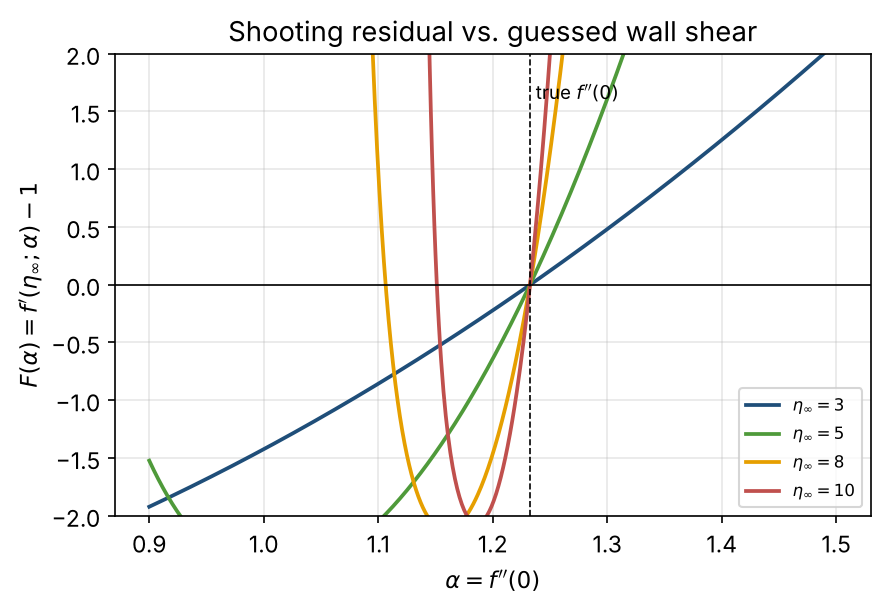
\includegraphics[width=0.68\textwidth]{shooting_landscape.png}
\caption{Shooting residual $F(\alpha)$ for several domain lengths. For $\eta_\infty=3$ the function
is monotone with a single root; for longer domains it becomes very steep and acquires spurious roots
to the left of the true value (dashed line). Values with $|F|>50$ (blown-up trajectories) are omitted.}
\label{fig:landscape}
\end{figure}

\begin{table}[H]
\centering
\caption{Converged $f''(0)$ from \texttt{solve\_ivp} shooting: Newton started at $\alpha_0=1$ on the
final domain versus continuation from $\eta_\infty=3$.}
\label{tab:cont}
\begin{tabular}{ccc}
\toprule
$\eta_\infty$ & Newton from $\alpha_0=1$ & with continuation \\
\midrule
3 & 1.23281554 & 1.23281554 \\
4 & 1.23259087 & 1.23259087 \\
5 & 0.85037098 & 1.23258768 \\
6 & 0.99593042 & 1.23258766 \\
8 & 1.10646364 & 1.23258766 \\
10 & 1.15117786 & 1.23258766 \\
\bottomrule
\end{tabular}

\end{table}

\subsection{Method 2: \texttt{solve\_ivp} integrator}
The augmented 6-equation system (state + sensitivity) is integrated with the adaptive
8th-order Dormand--Prince scheme (\texttt{DOP853}) at $\text{rtol}=10^{-10}$, $\text{atol}=10^{-12}$.
Newton stops when $|F| < 10^{-10}$.

\subsection{Method 3: hand-written RK4}
The same augmented system is advanced with the classical fixed-step RK4 scheme,
\begin{align*}
\mathbf{k}_1 &= \mathbf{g}(\eta_n,\mathbf{z}_n), &
\mathbf{k}_2 &= \mathbf{g}(\eta_n+\tfrac h2,\mathbf{z}_n+\tfrac h2\mathbf{k}_1),\\
\mathbf{k}_3 &= \mathbf{g}(\eta_n+\tfrac h2,\mathbf{z}_n+\tfrac h2\mathbf{k}_2), &
\mathbf{k}_4 &= \mathbf{g}(\eta_n+h,\mathbf{z}_n+h\mathbf{k}_3),\\
\mathbf{z}_{n+1} &= \mathbf{z}_n + \tfrac h6(\mathbf{k}_1+2\mathbf{k}_2+2\mathbf{k}_3+\mathbf{k}_4),
\end{align*}
with $h = 0.01$. Because the sensitivity is integrated by the same scheme, the Newton derivative is the
exact derivative of the discrete map, so quadratic convergence is retained. For plotting between nodes,
cubic Hermite interpolation is used with slopes taken from the ODE itself, which keeps the dense
output fourth-order accurate. No SciPy routines are used in this solver.

\section{Results}

\subsection{Comparison of methods}
\begin{table}[H]
\centering
\caption{Results at $\eta_\infty = 10$. Error is relative to the literature value $f''(0)=1.232587657$.
$\delta^* = \int_0^\infty (1-f')\,d\eta$ and $\theta = \int_0^\infty f'(1-f')\,d\eta$ are the
displacement and momentum thicknesses. Iteration counts for shooting are summed over all continuation stages.}
\label{tab:comp}
\small
\begin{tabular}{lcccccc}
\toprule
Method & $f''(0)$ & $|$Error$|$ & Iter. & $\delta^*$ & $\theta$ & Time (ms) \\
\midrule
solve\_bvp (collocation) & 1.23258766 & 1.9e-10 & 4 & 0.64790 & 0.29234 & 27.4 \\
solve\_ivp + Newton shooting & 1.23258766 & 1.8e-10 & 10 & 0.64790 & 0.29234 & 91.7 \\
Scratch RK4 + Newton shooting & 1.23258766 & 2.7e-10 & 10 & 0.64790 & 0.29234 & 295.7 \\
\bottomrule
\end{tabular}

\end{table}

All three methods agree to about $10^{-10}$ in $f''(0)$, i.e.\ to the precision with which the
reference value is quoted. The boundary-layer integrals are $\delta^* = \deltastar$ and
$\theta = \thetamom$ (shape factor $H = \delta^*/\theta \approx 2.22$), and $f'$ reaches
$0.99$ at $\eta_{99} \approx \etaninetynine$. The boundary-layer thickness is therefore constant
along the wall: the acceleration of the outer flow exactly balances viscous diffusion.
\texttt{solve\_bvp} is the fastest; the hand-written RK4 is slowest because it is a pure-Python loop with
a fixed, fine step.

\begin{figure}[H]
\centering
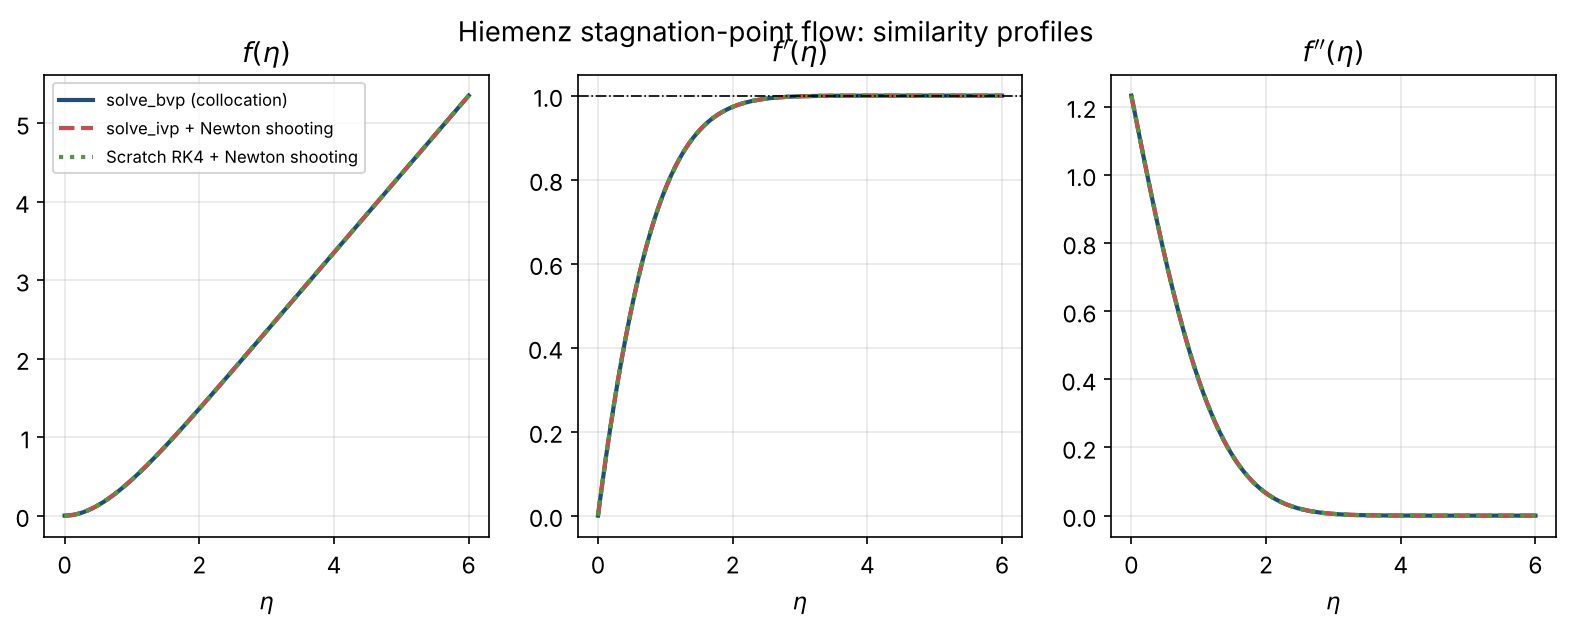
\includegraphics[width=\textwidth]{profiles.png}
\caption{Similarity profiles $f$, $f'$ (velocity $u/U_e$) and $f''$ (shear) from the three methods;
the curves are indistinguishable. $f$ becomes linear, $f \approx \eta - \delta^*$, outside the boundary layer.}
\label{fig:profiles}
\end{figure}

\begin{figure}[H]
\centering
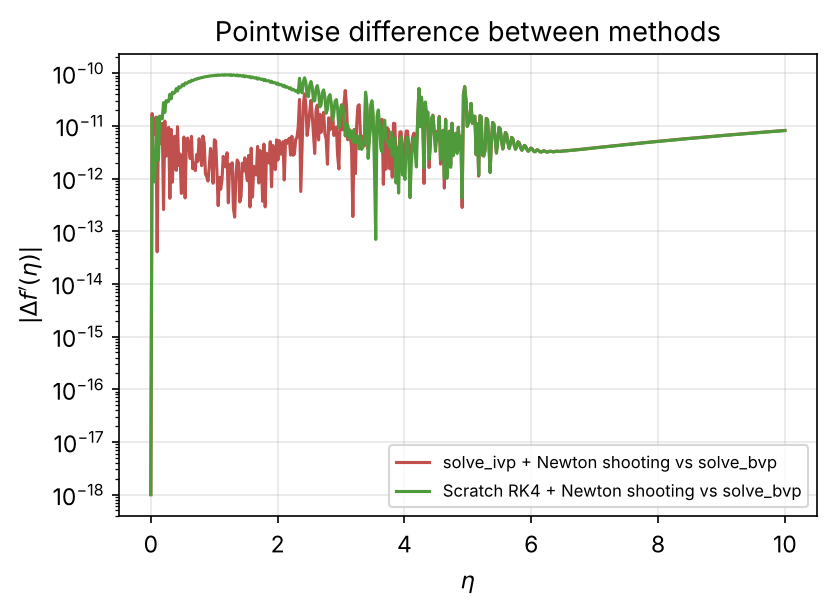
\includegraphics[width=0.62\textwidth]{method_difference.png}
\caption{Pointwise difference in $f'(\eta)$ between each shooting method and \texttt{solve\_bvp}.
Differences stay below $10^{-10}$ over the whole domain.}
\label{fig:diff}
\end{figure}

\subsection{Newton convergence}
Table~\ref{tab:newton} and Figure~\ref{fig:newton} show a single Newton solve on $\eta_\infty = 4$ from
$\alpha_0 = 1$. After the first two (damped) steps bring $\alpha$ into the basin of attraction, the
residual falls as $10^{-1}\to10^{-3}\to10^{-7}\to10^{-15}$: the number of correct digits roughly doubles
each iteration, the signature of quadratic convergence. Both integrators give the same history.

\begin{figure}[H]
\centering
\begin{minipage}{0.55\textwidth}
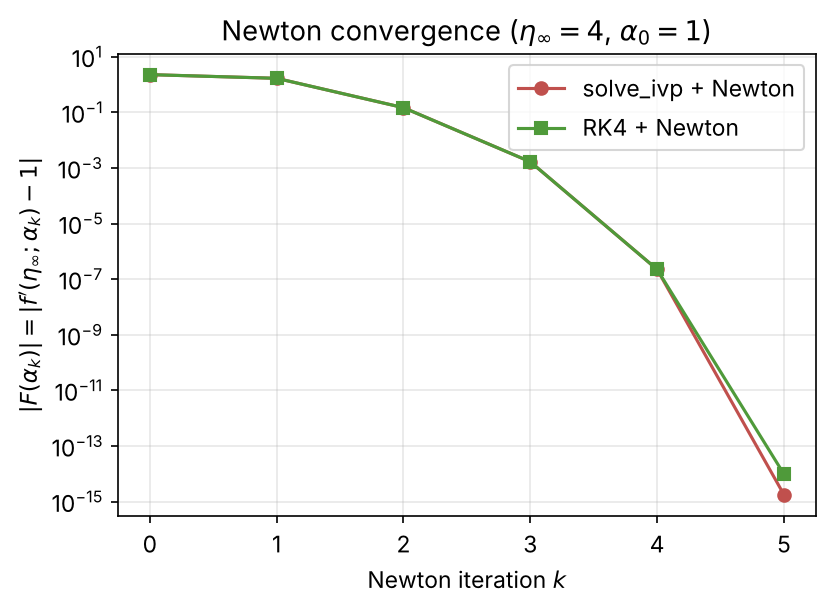
\includegraphics[width=\textwidth]{newton_convergence.png}
\captionof{figure}{Newton residual history.}
\label{fig:newton}
\end{minipage}\hfill
\begin{minipage}{0.42\textwidth}
\centering\small
\captionof{table}{Newton iterates (\texttt{solve\_ivp}, $\eta_\infty=4$).}
\label{tab:newton}
\begin{tabular}{ccc}
\toprule
$k$ & $\alpha_k$ & $|F(\alpha_k)|$ \\
\midrule
0 & 1.000000000000 & 2.270e+00 \\
1 & 1.348086763590 & 1.672e+00 \\
2 & 1.243847587727 & 1.472e-01 \\
3 & 1.232719844644 & 1.667e-03 \\
4 & 1.232590891267 & 2.238e-07 \\
5 & 1.232590873947 & 1.776e-15 \\
\bottomrule
\end{tabular}

\end{minipage}
\end{figure}

\subsection{Order of accuracy of RK4}
Figure~\ref{fig:rk4} plots the error in $f''(0)$ against step size, measured against a run with
$h = 0.0025$. A least-squares fit of $\log(\text{error})$ against $\log h$ gives slope
$\rkorder$, confirming the theoretical fourth-order accuracy of the scheme: halving $h$ reduces the error
by about $2^4 = 16$.

\begin{figure}[H]
\centering
\begin{minipage}{0.55\textwidth}
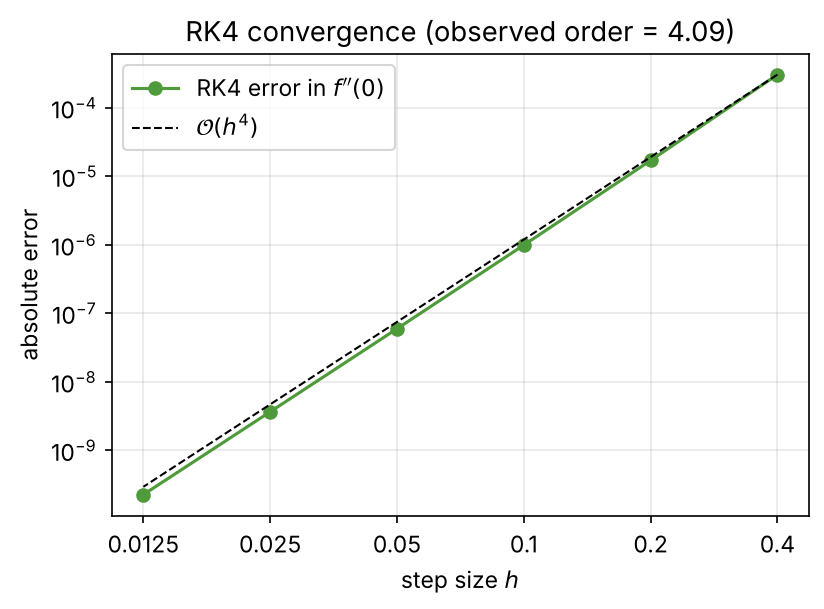
\includegraphics[width=\textwidth]{rk4_convergence.png}
\captionof{figure}{RK4 error versus step size.}
\label{fig:rk4}
\end{minipage}\hfill
\begin{minipage}{0.4\textwidth}
\centering\small
\captionof{table}{RK4 step-size study.}
\begin{tabular}{cc}
\toprule
$h$ & $|f''_h(0)-f''_{h\to0}(0)|$ \\
\midrule
0.4 & 3.072e-04 \\
0.2 & 1.713e-05 \\
0.1 & 9.949e-07 \\
0.05 & 5.970e-08 \\
0.025 & 3.652e-09 \\
0.0125 & 2.255e-10 \\
\bottomrule
\end{tabular}

\end{minipage}
\end{figure}

\subsection{Effect of the truncated domain length}
\label{sec:etainf}
Because $f' \to 1$ exponentially fast (like $e^{-\eta^2/2}$), the truncation error drops very quickly
with $\eta_\infty$ (Figure~\ref{fig:etainf}, Table~\ref{tab:etainf}). At $\eta_\infty=3$ the error is
$\sim 2\times10^{-4}$; by $\eta_\infty = 6$ it has fallen to the $10^{-10}$ level set by the solver
tolerances. Any $\eta_\infty \gtrsim 6$ is therefore sufficient; $\eta_\infty = 10$ is used as a safe default.
Truncating too \emph{late} does not harm collocation but makes shooting harder (Section~2.2).

\begin{figure}[H]
\centering
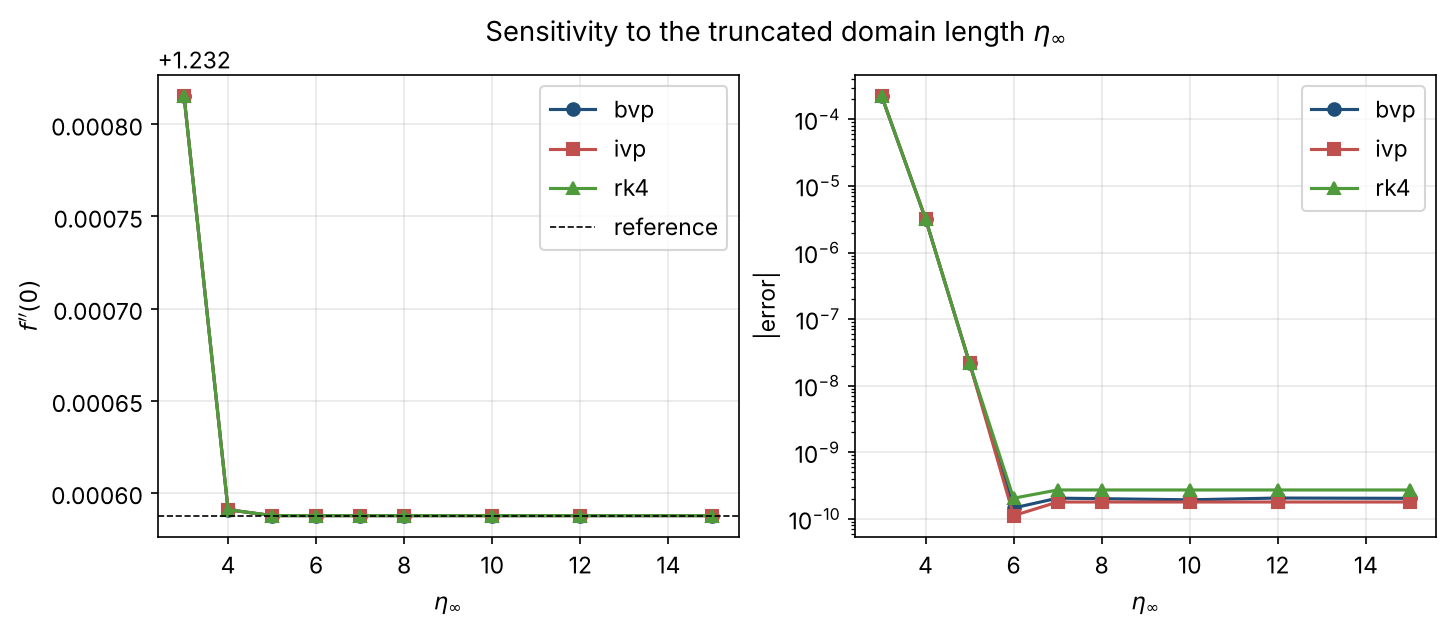
\includegraphics[width=\textwidth]{eta_inf_study.png}
\caption{Converged $f''(0)$ (left) and its error (right) as a function of $\eta_\infty$ for all three methods.}
\label{fig:etainf}
\end{figure}

\begin{table}[H]
\centering\small
\caption{$f''(0)$ versus domain length.}
\label{tab:etainf}
\begin{tabular}{cccc}
\toprule
$\eta_\infty$ & solve\_bvp & solve\_ivp + Newton & RK4 + Newton \\
\midrule
3 & 1.23281554 & 1.23281554 & 1.23281554 \\
4 & 1.23259087 & 1.23259087 & 1.23259087 \\
5 & 1.23258768 & 1.23258768 & 1.23258768 \\
6 & 1.23258766 & 1.23258766 & 1.23258766 \\
7 & 1.23258766 & 1.23258766 & 1.23258766 \\
8 & 1.23258766 & 1.23258766 & 1.23258766 \\
10 & 1.23258766 & 1.23258766 & 1.23258766 \\
12 & 1.23258766 & 1.23258766 & 1.23258766 \\
15 & 1.23258766 & 1.23258766 & 1.23258766 \\
\bottomrule
\end{tabular}

\end{table}

\section{Discussion and conclusions}
\begin{itemize}
\item All three methods give $f''(0) = 1.23258766$, $\delta^* = 0.6479$ and $\theta = 0.2923$,
in agreement with the classical Hiemenz solution.
\item \textbf{Collocation} (\texttt{solve\_bvp}) is the most robust and fastest: it treats both
boundaries simultaneously, so it is insensitive to the exponential error growth that affects shooting.
\item \textbf{Shooting} is simple and accurate, but for a semi-infinite domain it is ill-conditioned:
started from a poor guess on a long domain it converges to spurious roots. Continuation in
$\eta_\infty$ together with a damped Newton step makes it reliable.
\item Integrating the \textbf{variational equations} gives an exact Newton derivative, giving
quadratic convergence without the step-size trade-off of finite differences.
\item The hand-written \textbf{RK4} achieves its theoretical fourth-order accuracy (observed $\rkorder$)
and, with $h = 0.01$, matches the library solvers to $\sim10^{-10}$, at the cost of more run time.
\end{itemize}

\section*{Code}
Source code and instructions: see \texttt{README.md} in the repository.
Run \texttt{python main.py} to regenerate every figure and table in this report.

\begin{thebibliography}{9}
\bibitem{schlichting} H.~Schlichting and K.~Gersten, \emph{Boundary-Layer Theory}, 9th ed., Springer, 2017.
\bibitem{white} F.~M.~White, \emph{Viscous Fluid Flow}, 3rd ed., McGraw-Hill, 2006.
\bibitem{scipy} P.~Virtanen \emph{et al.}, ``SciPy 1.0: fundamental algorithms for scientific computing in Python,'' \emph{Nature Methods} 17, 261--272 (2020).
\end{thebibliography}
\end{document}
